\begin{frame}[fragile]{Uso de Text-to-Speech (TTS) en Android}
\textbf{¿Qué es Text-to-Speech (TTS)?}

\begin{itemize}
    \item Es una tecnología que convierte texto en voz sintetizada.
    \item Permite a una aplicación "hablar" al usuario.
    \item Útil en accesibilidad, asistentes virtuales y notificaciones.
\end{itemize}


\textbf{Pasos básicos:}
\begin{itemize}
    \item Crear una instancia de \texttt{TextToSpeech}.
    \item Configurar idioma y velocidad.
    \item Invocar el método \texttt{speak()} para reproducir el texto.
\end{itemize}


\textbf{Consideraciones:}
\begin{itemize}
    \item Verificar que el idioma esté soportado.
    \item Liberar recursos con \texttt{tts.shutdown()} en \texttt{onDestroy()}.
    \item Requiere motor TTS instalado en el dispositivo.
\end{itemize}

\end{frame}



\begin{frame}[fragile]
\frametitle{Demo 14: Text to Speech (TTS) }
\begin{columns}
\column{0.80\linewidth}
Del Repositorio Github:
\begin{itemize}
\item Copiar el archivo \textit{MainActivity\_Demo14.java} (dentro del Folder códigosJAVA) al mismo directorio donde esta el MainActivity.java
\item Copiar el archivo \textit{activity\_main\_demo14.xml} (dentro del Folder Carpeta\_layout) al mismo directorio donde esta el activity\_main.xml
%\item Copiar el archivo \textit{custom\_dialog.xml} (dentro del Folder Carpeta\_layout) al mismo directorio donde esta el activity\_main.xml.
\item Modificar en el archivo \textit{AndroidManifest.xml} la cadena \textit{.MainActivity\_Demo13} por \textit{.MainActivity\_Demo14}.
%\item Agregar la siguiente linea: \textit{implementation (``com.journeyapps:zxing-android-embedded:4.3.0'')}, al final de la seccion Dependencies del archivo Build.graddle.kts (Module: App).

%\item Ir a la linea 22 de archivo del archivo \textit{MainActivity\_Demo09.java}, poner el cursos en la palabra (en Rojo) \textit{documentfile}, presionar la combinación ALT+ENTER, y seleccionar de la lista desplegable la opcion ``Add dependency on ....''. Esto quitará el error y hara los ajustes necesarios. 
\end{itemize}

%\begin{block}{Demo \#09}
%Un App que permite escribir el contenido de un EditText a un archivo y cargar el contenido de cualquier archivo en el EditText
%\end{block}


\column{0.20\linewidth}

\begin{center}
 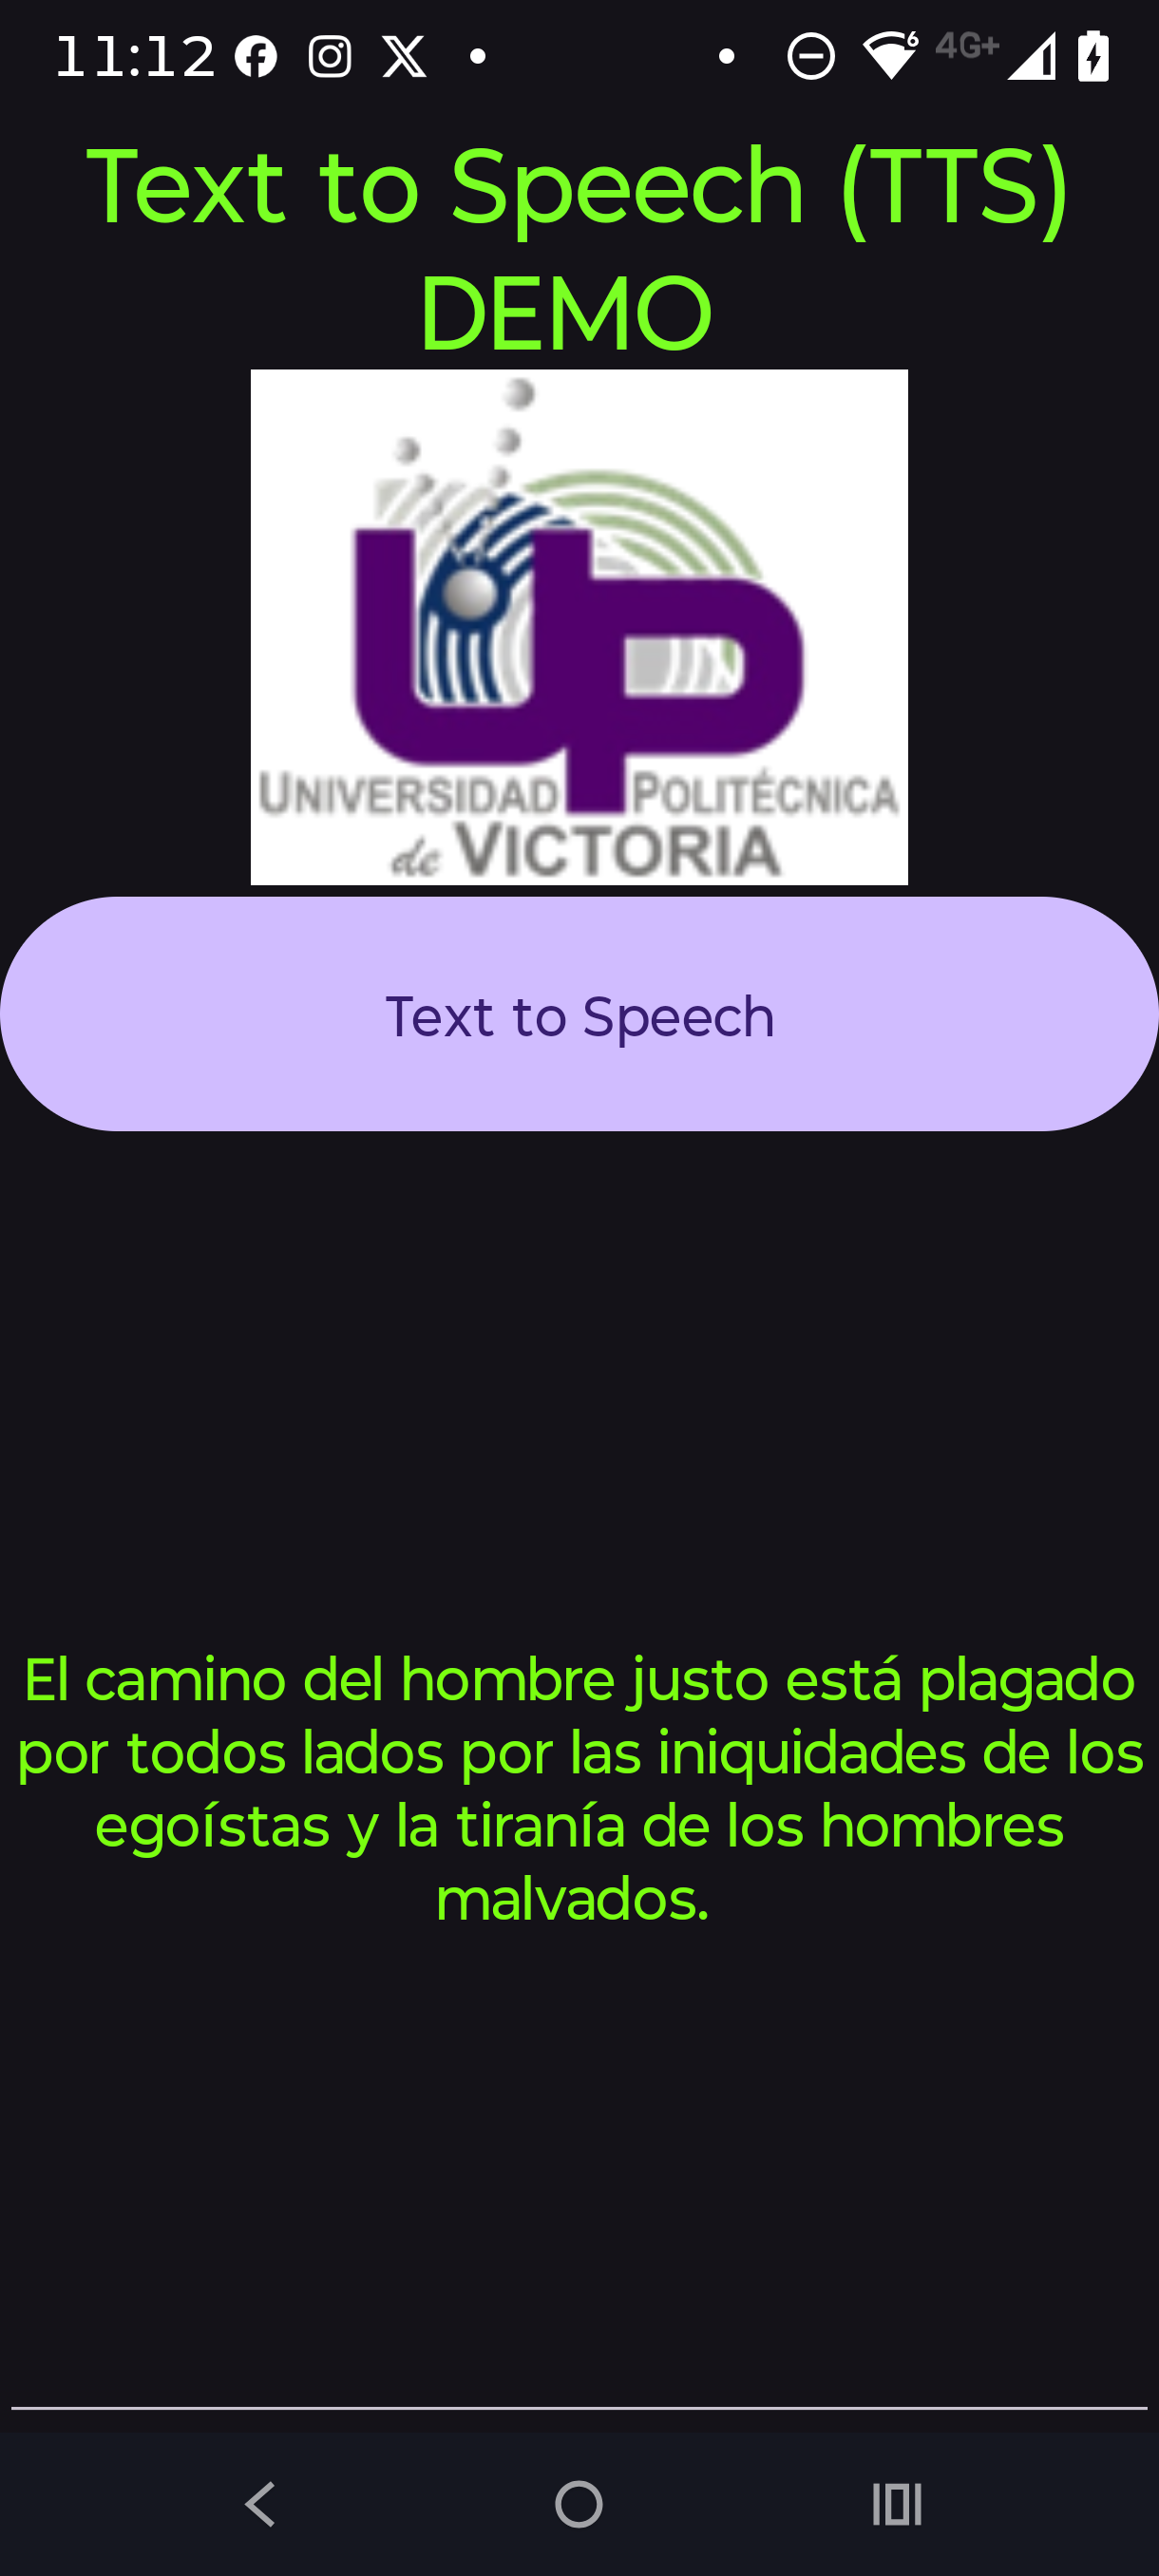
\includegraphics[width=0.98\textwidth]{02_TallerCBTis/figs/Demo14}
\end{center}

\end{columns}

\end{frame}

